\setcounter{page}{0}
\chapter{\chapternameintro} \label{introduction}

\section{Galáxias}\label{sec:Galaxias}
As galáxias são sistemas gravitacionalmente ligados, compostos por matéria bariônica e não bariônica: estrelas, gás, poeira e matéria escura. Elas estão presentes no universo observável em diversos tamanhos e formas, desde as anãs até as gigantes. Elas são a base para a cosmologia e parte fundamental para entender a evolução do universo. São peças que reconstituem os blocos de formação do universo, e dessa forma conectam o entendimento desde as estruturas de menor escala, como nosso próprio sistema estelar, até as maiores estruturas do universo.

Nas últimas décadas, com o desenvolvimento de novos instrumentos na área observacional (e.g., \citealp{hubble_classification_1926}, \citealp{VLT_2010}, \citealp{JWT_2006}), foi possível compreender melhor os mecanismos de formação e evolução das galáxias. Com os novos levantamentos de dados, maior profundidade e melhoria na qualidade das observações, temos em mãos grandes catálogos com milhões de galáxias observadas, presentes em diversos ambientes e em diferentes épocas do universo (e.g., \citealp{SDSS_2000}, \citealp{COSMOS_2007}, \citealp{DES_2018}, \citealp{oliveira2019splus}). Além disso, houve avanços nos modelos e simulações, com melhores softwares e hardwares, possibilitando análises mais detalhadas dos dados e permitindo validar os modelos teóricos (e.g., \citealp{Vogelsberger_2014}, \citealp{EAGLE_2015}).

Uma das dificuldades que temos é modelar como as galáxias se formam ao longo do tempo, necessitando de um melhor entendimento dos processos internos em pequena e larga escala. Atualmente, acreditamos que a formação das galáxias começou a partir de pequenas flutuações no campo de densidade primordial do universo, que foram evoluindo após o início do Big Bang \citep{liddle_1999}. Assim, as estruturas do universo foram surgindo de forma hierárquica, com as galáxias mais massivas se formando a partir das menores, por meio de fusões e interações gravitacionais.

Nesta seção, falarei brevemente sobre o entendimento da formação de galáxias. Além disso, discutirei os tipos de galáxias mais massivas e, principalmente, os tipos das galáxias anãs. Nas próximas seções, tratarei sobre as propriedades e cenários de formação do objeto de interesse deste trabalho, as galáxias anãs ultra-compactas ({\it ultra compact dwarfs}, UCDs).

\subsection{Modelos de formação de Galáxias}\label{subsec:modelo_formacao_galaxias}

Tratando dos modelos de formação de galáxias, o modelo padrão cosmológico mais utilizado atualmente é o modelo $\Lambda$ Cold Dark Matter ($\Lambda CDM$), que propõe que o universo é constituído principalmente por matéria escura fria ({\it cold dark matter}, CDM) e energia escura, na forma de uma constante cosmológica $\Lambda$. A matéria escura ser chamada de fria se refere a ela se mover lentamente comparada à velocidade da luz. No modelo $\Lambda CDM$, as estruturas se formam hierarquicamente, em que primeiro os objetos menores são formados para então se fundirem e se transformarem em halos maiores \citep{Blumenthal_1984}.

Considerando que o universo teve início no Big Bang, se expandindo e esfriando, as primeiras flutuações de densidade surgiram devido a flutuações quânticas no campo de densidade primordial \citep{liddle_1999}. No começo, o universo era constituído por um plasma quente e denso composto de fótons e matéria, que foi se expandindo e esfriando lentamente. Com o tempo, ele atingiu valores de densidade e temperaturas suficientemente baixos para permitir que os primeiros átomos estáveis se formassem, principalmente o hidrogênio neutro.

O que conhecemos como radiação cósmica de fundo (CMB) é a radiação eletromagnética liberada quando o universo, que já estava suficientemente frio para que os átomos se formassem, se tornou transparente. Os fótons foram desacoplados da matéria bariônica, propagando-se e formando a radiação que observamos hoje em dia, que permeia todo o universo. Com o modelo $\Lambda CDM$, as flutuações no campo de densidades da CMB são as sementes para poder criar as estruturas maiores. De acordo com medições do CMB, principalmente com os levantamentos de dados mais recentes, como o \textit{Planck} \citep{Planck_2020}, o universo tem cerca de 13.8 Gyr, e é composto de energia escura em uma fração de $\Omega_\Lambda \sim 0.7$, de matéria escura com $\Omega_{DM} \sim 0.25$, e de bárions com $\Omega_b \sim 0.05$.

Na cosmologia $\Lambda CDM$, as primeiras estruturas se formam a partir do colapso gravitacional de sobredensidades primordiais. Para descrever os eventos subsequentes de formação de galáxias até hoje, podemos observar as evoluções de acordo com o desvio para o vermelho (redshift - $z$).

Em valores de $z$ entre 10 e 30, os bárions conseguiram se manter nos primeiros halos de matéria escura formados no universo, e dentro deles surgiram as primeiras estrelas das galáxias (e.g., \citealp{Glover_2005}, \citealp{Greif_2015}, \citealp{Schauer_2021}). As primeiras estrelas, conhecidas como estrelas de população III, eram compostas apenas de hidrogênio e hélio, sendo muito massivas e brilhantes. A radiação que elas produziram ionizou o hidrogênio ao seu redor, e em um $z \sim 6-10$, essa ionização do hidrogênio marcou o final da época da reionização \citep{Wise_2019}. As galáxias começaram a se formar e evoluir ainda durante a época da reionização, com a formação de estrelas e a evolução de suas populações estelares. As estruturas maiores, como aglomerados e superaglomerados, também começaram a se formar a partir de fusões e interações gravitacionais. Sob influência gravitacional, elas evoluem e se fundem, formando as estruturas em larga escala.

Juntamente com o modelo cosmológico $\Lambda CDM$, temos a origem das galáxias a partir da formação hierárquica. Pelas simulações cosmológicas, que utilizam a dissipação de gás e física bariônica junto da matéria escura, temos um esquema de formação em duas fases (e.g., \citealp{Oser_2010}, \citealp{Pillepich_2014}). Na primeira, as estrelas se formam na própria galáxia a partir do gás presente no halo de matéria escura. Depois, a galáxia cresce ao incorporar galáxias satélites por meio de fusões. Observamos na nossa galáxia o crescimento dela via fusões, vendo as galáxias satélites, por exemplo, que estão sendo acrecidas ou mesmo as estrelas de correntes mareais que são deixadas por essas fusões. Nas correntes mareais, observamos estrelas que foram retiradas de galáxias menores que foram acrecidas pela galáxia principal, em que a galáxia original foi destruída e suas estrelas se espalharam ao longo do tempo. Um desses exemplos visto na nossa galáxia é a corrente de Sagitário, que é uma corrente mareal deixada pela galáxia anã de Sagitário, que está sendo acrecida pela Via Láctea.

Nas galáxias mais distantes, é ainda mais complicado observar essas correntes devido ao seu baixo brilho superficial. Porém, para galáxias externas, as melhores evidências de fusões moldando galáxias vêm das observações de sistemas atualmente interagindo, que muitas vezes mostram morfologias e cinemáticas perturbadas.

Nas estruturas em larga escala que observamos, encontramos a teia cósmica, que é composta por filamentos, vazios e nós. Os filamentos, formados por matéria escura e galáxias ao longo deles, conectam os nós, que são os aglomerados de galáxias mais massivos. Entre os filamentos, encontram-se as regiões de vazios, que são áreas com baixa densidade de matéria e galáxias \citep{Lindner_1995}. Com as observações atuais, podemos recuperar e reconstruir a distribuição de galáxias e mapear essa teia cósmica (\citealp{Lindner_1995}, \citealp{Abazajian_2003}), observando que as propriedades estão de acordo com os resultados de simulações cosmológicas, marcando um dos grandes sucessos para o modelo $\Lambda CDM$.

Apesar do sucesso do $\Lambda CDM$, ainda há problemas e teorias alternativas propostas. As naturezas da matéria escura e da energia escura ainda precisam ser explicadas, e há algumas inconsistências em pequenas e grandes escalas. Um dos problemas é o dos satélites ausentes na nossa galáxia (\citealp{Klypin_1999}, \citealp{Moore_1999}). Embora com o aumento dos estudos e descobertas de novos satélites, ainda haja uma diferença entre o número de satélites observados e o número previsto pelas simulações. Porém, não está claro se é uma ausência real ou apenas a não detecção ainda desses halos. A falta de pequenas estruturas implica que a formação de galáxias ocorre em subhalos da Via Láctea, mas essas estruturas são menos densas do que o esperado nas simulações \citep{Boylan_Kolchin_2011}. Essas dificuldades fizeram com que alguns considerassem cenários cosmológicos alternativos. Alguns envolvem inflação não padrão (e.g., \citealp{Kamionkowski_2000}), outros de matéria escura não fria (e.g., \citealp{Murgia_2017}), por exemplo. Porém, o modelo $\Lambda CDM$ ainda é o mais aceito e bem-sucedido para explicar a formação e evolução do universo, e tem sido altamente bem-sucedido na reprodução de observações em escalas maiores do que alguns kpcs.


\subsection{Galáxias Early e Late - type}\label{subsec:Galaxia_early_late}
Em 1926, Edwin Hubble criou um dos primeiros esquemas para a classificação de galáxias, dividindo-as em categorias que abrangiam uma maior quantidade de objetos: galáxias elípticas, lenticulares e espirais \citep{hubble_classification_1926}. As galáxias elípticas são caracterizadas por sua forma esferoidal e, de forma geral, cessaram sua formação estelar, possuindo uma população estelar mais velha e com menos gás e poeira. Juntamente com as lenticulares (S0), que diferem das elípticas por terem um disco de estrelas e gás, mas sem a presença de braços espirais, são conhecidas como galáxias early-type.

Já as espirais são caracterizadas por terem um disco de estrelas e gás, com braços espirais e um bojo central, e são conhecidas como galáxias late-type. Na Figura \ref{hubble_sequence}, é possível observar a sequência de Hubble, que mostra a classificação de galáxias de acordo com sua morfologia. Na Figura \ref{galaxies_morphology}, é possível ver exemplos de galáxias de diferentes tipos morfológicos, na mesma ordem apresentada na Figura \ref{hubble_sequence}, para exemplos de galáxias \textit{E0}, \textit{S0} e \textit{Irregular}. Fora desse esquema de classificação, temos as galáxias de baixa massa, que apresentam morfologias mais irregulares.

\begin{figure}[!ht]
    \begin{center}
    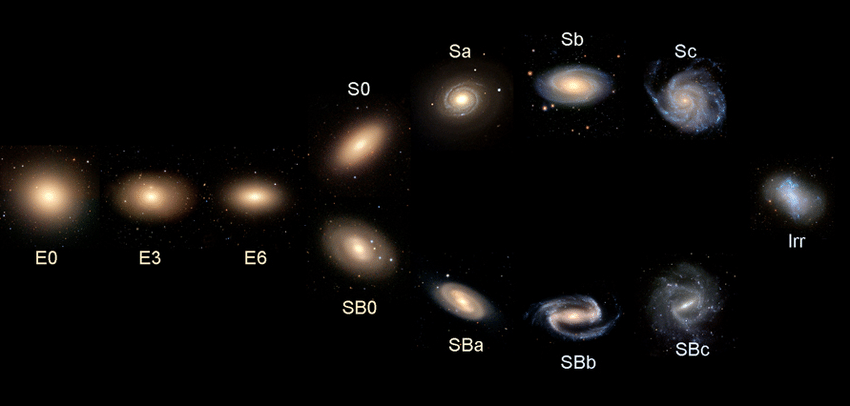
\includegraphics[width=0.7\columnwidth,angle=0]{indroduction/hubble_sequence.png}
    \caption[]{Sequência de Hubble, mostrando a classificação de galáxias de acordo com a morfologia. Créditos: \cite{huble_sequence_img}.}
    \label{hubble_sequence}
    \end{center}
\end{figure}


\begin{figure}[!ht]
    \centering
    \captionsetup{justification=centering}
    \begin{subfigure}[b]{0.237\textwidth}
        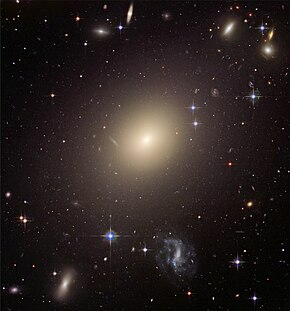
\includegraphics[width=\textwidth]{indroduction/E0_ex.png}
        \caption{}
    \end{subfigure}
    \begin{subfigure}[b]{0.26\textwidth}
        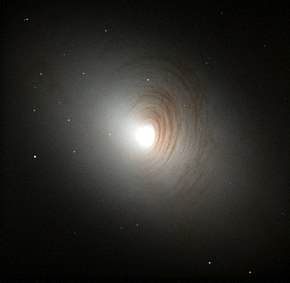
\includegraphics[width=\textwidth]{indroduction/S0_ex.png}
        \caption{}
    \end{subfigure}
    \begin{subfigure}[b]{0.268\textwidth}
        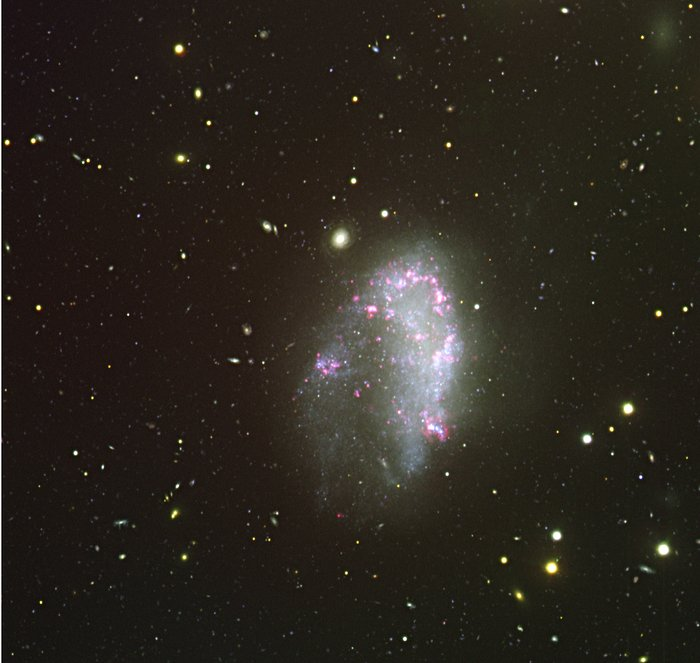
\includegraphics[width=\textwidth]{indroduction/irregular_ex.png}
        \caption{}
    \end{subfigure}
    \caption{Exemplos de diferentes tipos morfologios de galáxias. a) Early-type (E0) ESO 325-4, b) Lenticular (S0) NGC 2787, c) Irregular NGC 1427. Créditos: a) NASA/ESA, b) NASA/ESA, c) ESO.}
    \label{galaxies_morphology}
\end{figure}


\subsection{Galáxias anãs}\label{subsec:}
As galáxias anãs estão presentes no universo em diversos formatos, com diferentes tipos de estruturas e composições. Elas representam a categoria mais numerosa no universo, dada sua diversidade. Esse tipo de galáxia é também caracterizado pela baixa luminosidade, como o nome sugere, sendo muito menos luminosas e menores do que suas companheiras maiores apresentadas anteriormente.

O limite exato para categorizá-las é incerto, não sendo uniformemente definido. Suas massas normalmente são encontradas com valores entre $10^5$ e $10^9$ massas solares. Os critérios de classificação entre as próprias galáxias anãs, inicialmente, também seguiam os exemplos observacionais de suas morfologias, assim como o brilho superficial \citep{dwarf_classification_init}. Porém, ao longo das melhorias dos dados observacionais, que até então para sistemas menores e mais fracos eram limitados, surgiram novos critérios que levam em conta características como a cinemática interna. Além disso, a distinção entre os tipos de galáxias anãs a partir do meio interestelar também é um critério importante, utilizando a presença de gás e poeira para diferenciá-las.

Sobre as galáxias anãs com pouca quantidade de gás, parte do fato disso acontecer é por causa das interações com galáxias maiores, que podem remover o gás de galáxias anãs, impedindo a formação de novas estrelas. Além disso, a pressão de radiação e os ventos estelares das estrelas mais massivas podem tirar o gás de galáxias anãs, e no geral o meio interestelar delas tem dificuldade de manter o gás. As galáxias anãs de menor massa fazem parte desse grupo e, devido às suas baixas luminosidades, foram primeiramente localizadas nas regiões mais próximas, no Grupo Local. Elas se dividem em dois principais grupos: \ac{dSph} e \ac{dE}. Das mais massivas desse grupo, as anãs elípticas, com as observações em aglomerados de galáxias, foram descobertas e inicialmente colocadas como uma categoria separada de galáxias mais massivas, sendo bem diferentes das suas contrapartes locais. Porém, a partir do início dos estudos de \cite{Forbes_2011}, foi sugerida uma transição contínua entre os tipos \ac{dSph} e \ac{dE}.

Da categoria das galáxias anãs com maior conteúdo de gás, temos as anãs compactas azuis, conhecidas como \ac{BCD}, e as anãs irregulares, conhecidas como \ac{dIrr}. Pela presença de gás, essas galáxias apresentam formação estelar contínua. No caso das BCDs, elas apresentam surtos de formação estelar fortes, que duram um menor tempo \citep{Thornley2000}, enquanto as dIrrs apresentam formação estelar prolongada, porém em baixas taxas \citep{McQuinn2010}.

Quando falamos do grupo de baixa massa e luminosidade, mesmo dentro do grupo das galáxias anãs, temos as \ac{UDG}. Por serem tão difusas, seus tamanhos podem ser comparados com algumas galáxias massivas, porém têm massas muito baixas, cerca de $10^7$ massas solares \citep{van_Dokkum2015}. 

Por serem difusas, de baixa massa e baixa luminosidade, são extremamente difíceis de detectar e observar. Sendo um dos extremos dos grupos de massas das galáxias, são um desafio para os modelos padrão e podem ajudar a entender a formação e evolução de galáxias, assim como a distribuição da matéria escura.

Por fim, temos as galáxias anãs ultra-compactas (UCDs), que são a categoria e parte deste trabalho na busca por novos objetos. Comentaremos mais sobre as UCDs na próxima seção, abordando sua origem, localização, cenários de formação e propriedades, além de como elas se correlacionam com outro tipo de objeto conhecido como aglomerados estelares nucleares (\ac{NSC}).

Apresentamos na Figura \ref{dwarf_galaxies} exemplos de galáxias anãs de diferentes tipos morfológicos: a primeira imagem mostra uma galáxia anã esferoidal (dSph), a segunda uma galáxia anã elíptica (dE), a terceira uma galáxia anã irregular (dIrr) e a quarta uma galáxia anã compacta azul (BCD).


\begin{figure}[!ht]
    \centering
    \captionsetup{justification=centering}
    \begin{subfigure}[b]{0.33\textwidth}
        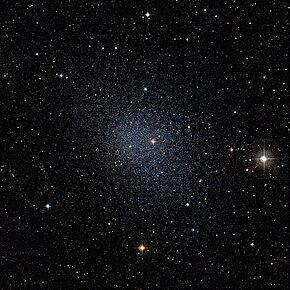
\includegraphics[width=\textwidth]{indroduction/dSph.png}
        \caption{}
    \end{subfigure}
    \begin{subfigure}[b]{0.33\textwidth}
        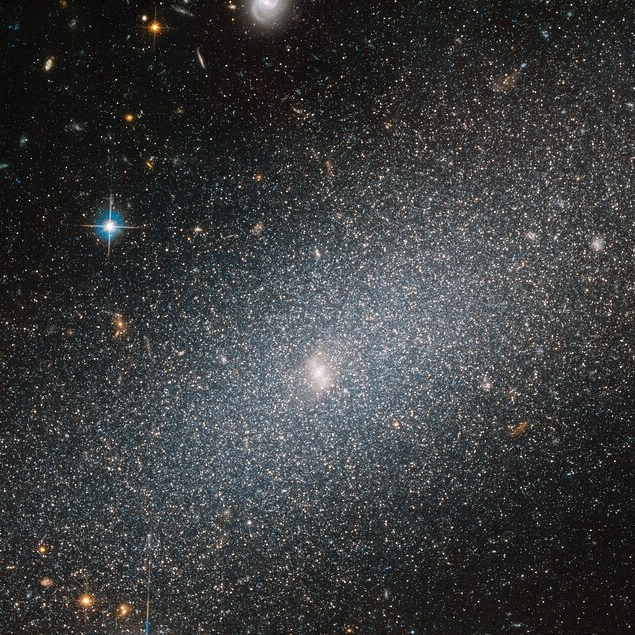
\includegraphics[width=\textwidth]{indroduction/dE.png}
        \caption{}
    \end{subfigure}
    \begin{subfigure}[b]{0.33\textwidth}
        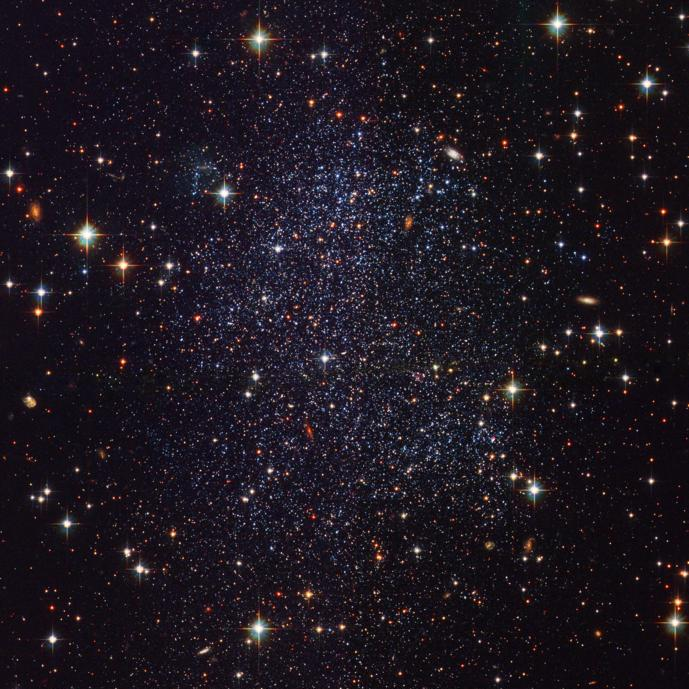
\includegraphics[width=\textwidth]{indroduction/dIrr.png}
        \caption{}
    \end{subfigure}
    \begin{subfigure}[b]{0.33\textwidth}
        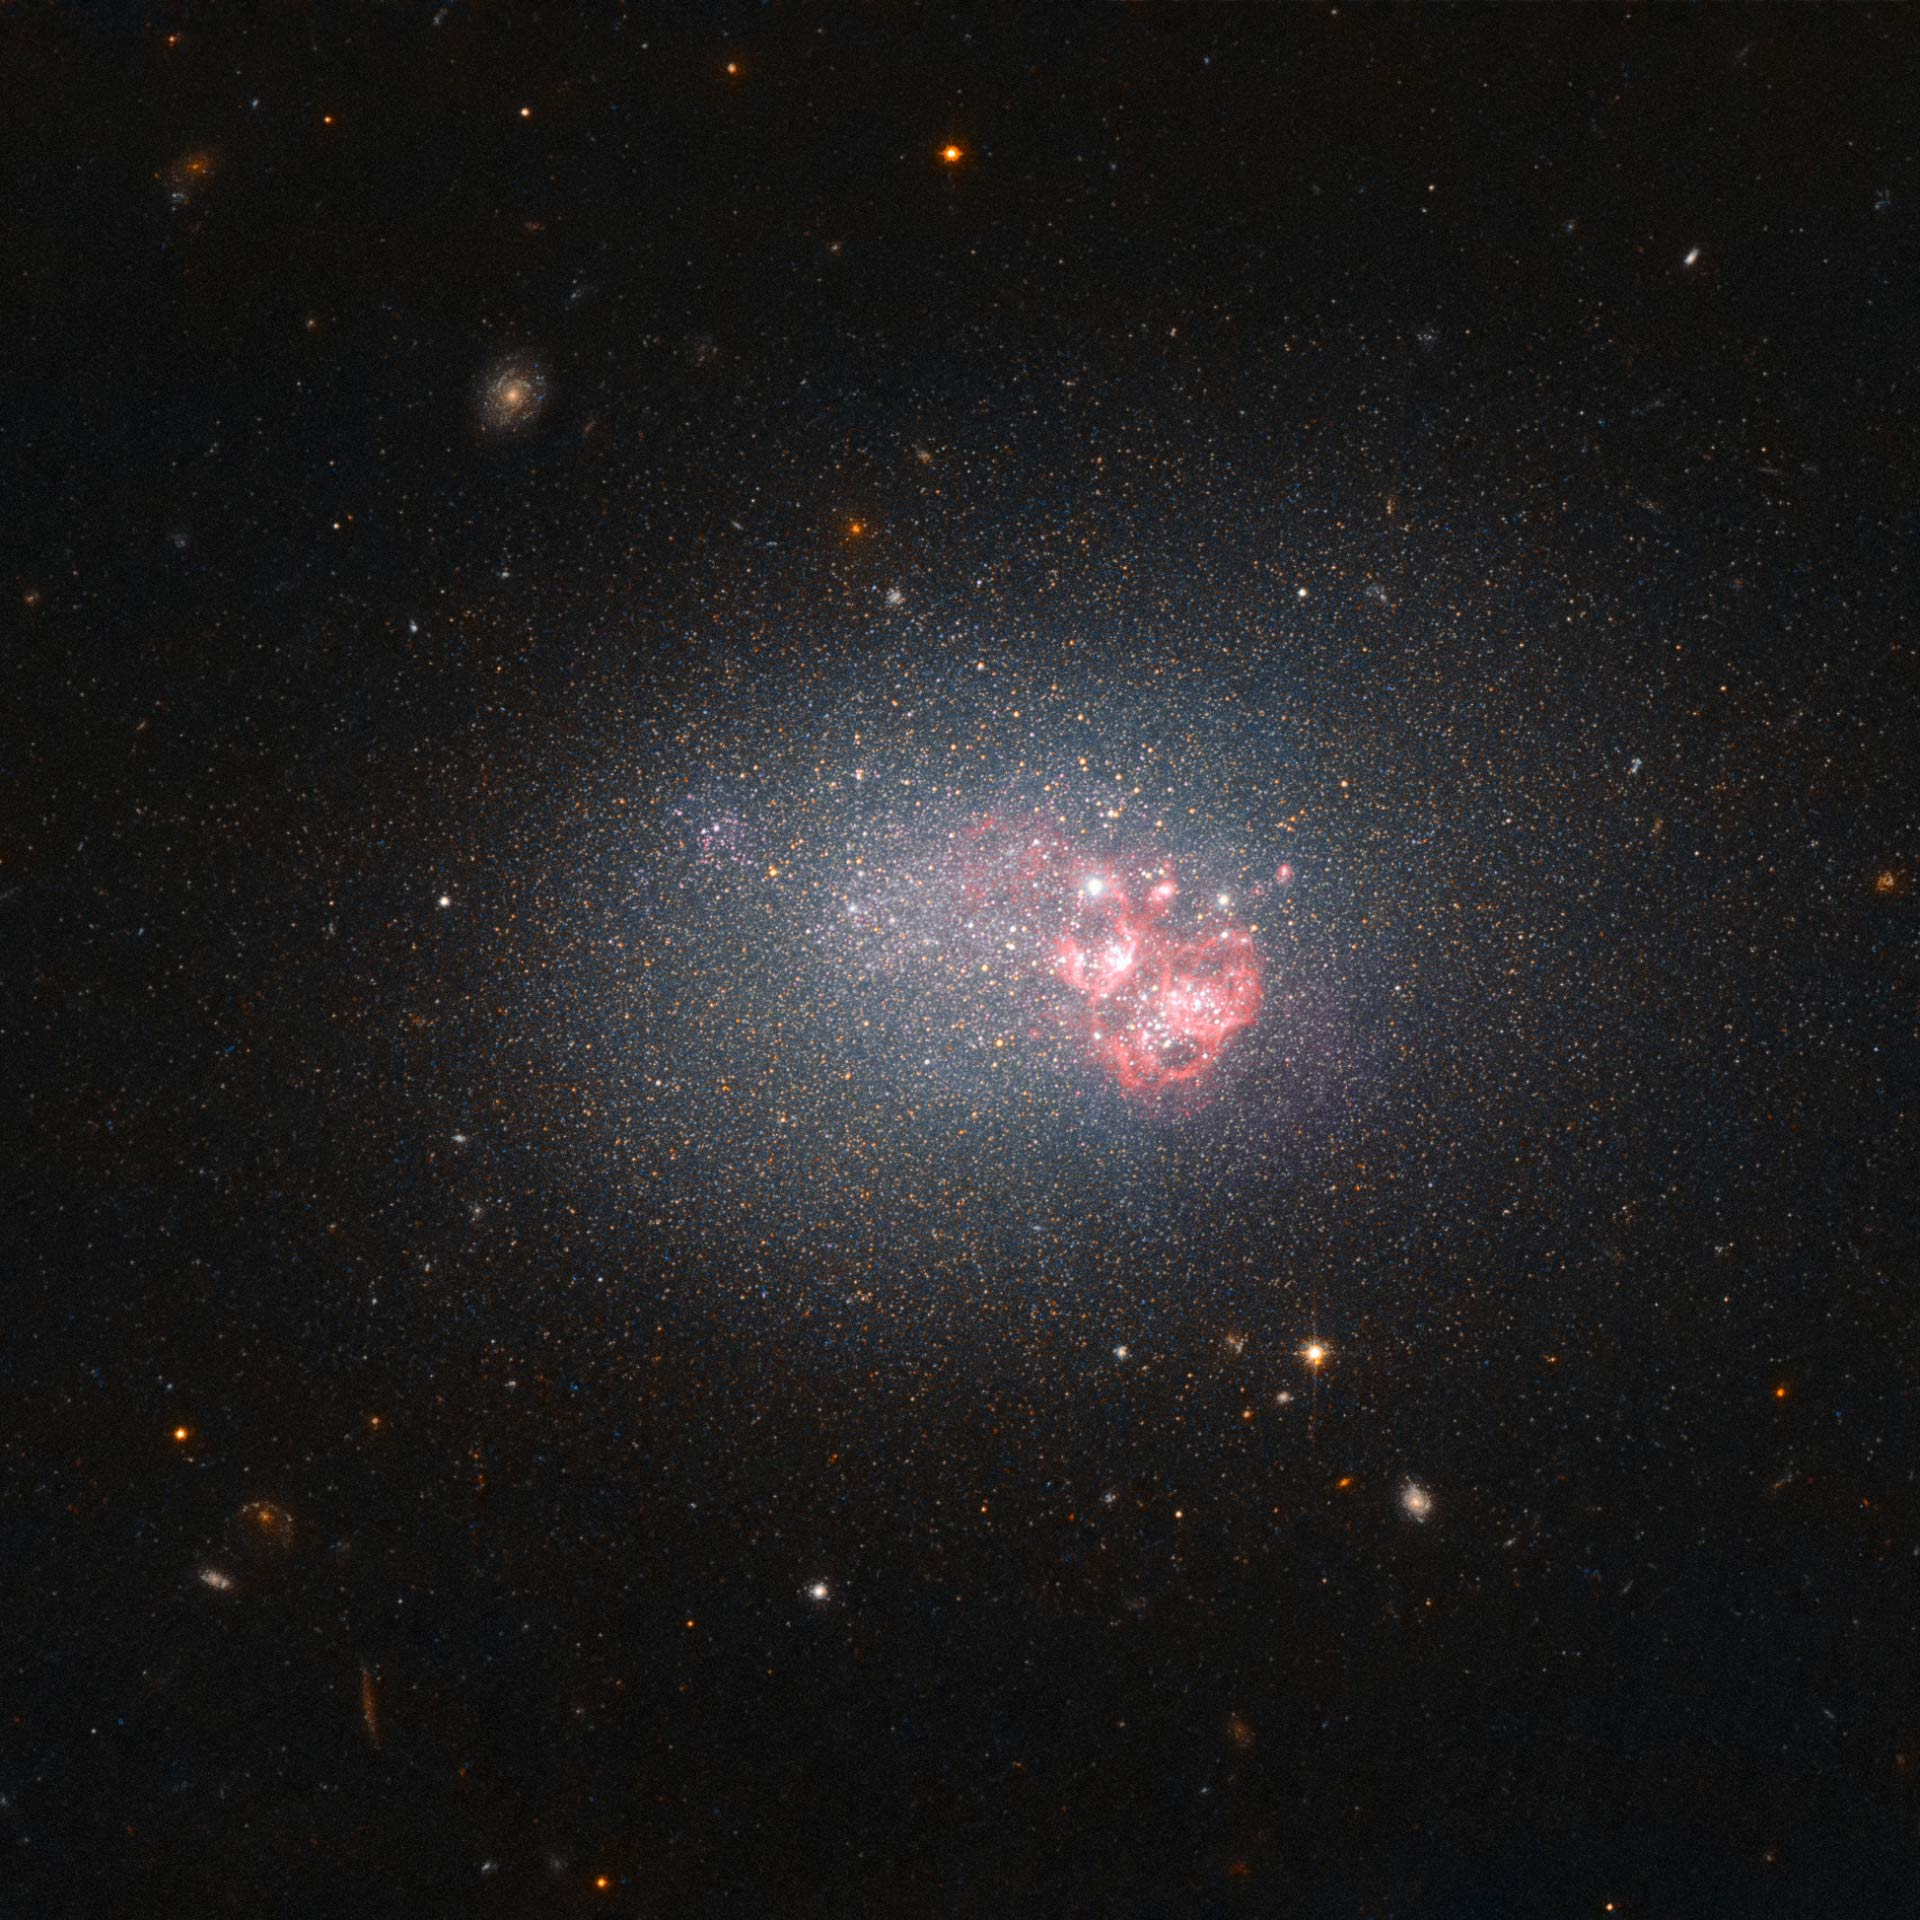
\includegraphics[width=\textwidth]{indroduction/BCD.png}
        \caption{}
    \end{subfigure}
    \caption{Exemplos de diferentes tipos morfologios de galáxias anãs conhecidas. a) Anã esferoidal (dSph) Fornax Dwarf Spheroidal, b) Anã elíptica (dE) PGC 29388, c) Anã irregular (dIrr) SagDIG, d) Anã compacta azul (BCD) LEDA 17302. Créditos: a) ESO/Digitized Sky Survey 2, b) ESA/Hubble, c)NASA, ESA, and The Hubble Heritage Team (STScI/AURA), d) NASA/ESA/Hubble.}
    \label{dwarf_galaxies}
\end{figure}


\section{UCDs}\label{sec:UCDs}
As galáxias anãs ultra-compactas são um tipo de objeto que se encontra entre as galáxias anãs e os \ac{GC}. Elas foram inicialmente descobertas em levantamentos de dados espectroscópicos no aglomerado de Fornax por \citealp{Drinkwater_2000} e \citealp{Hilker_1999}. Desde sua descoberta, passaram a ser encontradas em outros aglomerados e grupos de galáxias, como em Virgo (\citealp{Hasegan_2005} e \citealp{Liu_2020}), Abell 1689 \citep{Mieske_2005}, Centaurus \citep{Mieske_2007}, Hydra \citep{Wehner_Harris_2007}, Abell S0740 \citep{Blakeslee_DeGraaff2008}, no grupo NGC 1023 \citep{Mieske_West_Oliveira_2007}, no Grupo Dorado \citep{Evstigneeva_2007}, no grupo NGC 5044 \citep{Faifer_2017}, no grupo NGC 3613 \citep{Bortoli_2020}, e no grupo fóssil NGC 1132 \citep{Madrid_2011}. Além de já terem sido encontradas ao redor de galáxias isoladas \citep{Hau_2009}.

Até o final dos anos 2000, acreditava-se que as divisões entre sistemas classificados como aglomerados estelares ou galáxias eram mais rígidas. Devido às controvérsias sobre suas origens, elas também já foram chamadas de objetos ultracompactos (UCOs) \citep{Mieske_2002} e de objetos de transição globular-anão (DGTOs) \citep{Hasegan_2005}. As galáxias eram categorizadas pela presença de matéria escura e iam dos tamanhos de quiloparsecs, enquanto os aglomerados estelares eram considerados conjuntos de estrelas com raios de poucos parsecs, sem a presença de matéria escura. Porém, com a descoberta das UCDs, essa divisão tornou-se mais complicada, pois apresentam características de ambos os grupos, sendo inicialmente considerados objetos intermediários.

Mesmo com a crescente descoberta de novas UCDs e com trabalhos que abordam tanto a origem quanto a evolução e as características presentes nelas, o processo de formação das UCDs continua controverso. Abordaremos com mais detalhes os cenários de formação das UCDs na seção \ref{subsec:formacao}. Resumidamente, as teorias principais da sua formação vão em duas direções: a formação de UCDs a partir de galáxias anãs que passaram por processos de stripping e a formação de UCDs a partir de aglomerados globulares massivos. Porém, as evidências mais fortes sobre o tópico mostram que nenhum cenário de formação de UCDs é responsável por todas as populações conhecidas desses objetos. Uma mistura de processos pode ser a solução, com mais de um canal de formação, explicando suas diversidades de propriedades já observadas.

Mostramos na Figura \ref{UCDs_exp} exemplos de galáxias anãs ultra-compactas encontradas em diferentes ambientes, sendo a primeira imagem uma UCD encontrada próxima a M60, a segunda uma UCD encontrada próxima a M87 e a terceira uma UCD encontrada próxima a NGC 1399, no aglomerado de Fornax.

\begin{figure}[!ht]
    \centering
    \captionsetup{justification=centering}
    \begin{subfigure}[b]{0.3\textwidth}
        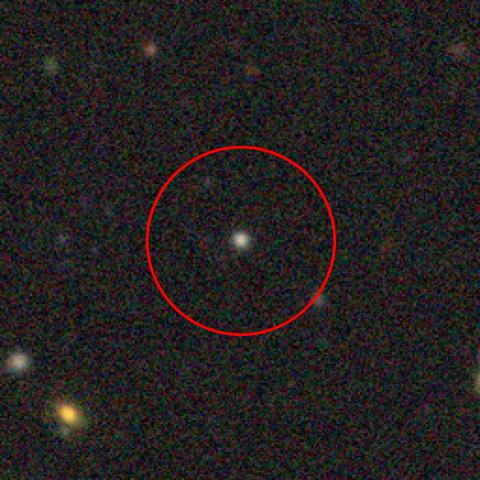
\includegraphics[width=\textwidth]{Images/ucds_exp/UCD_M60.png}
        \caption{}
    \end{subfigure}
    \begin{subfigure}[b]{0.3\textwidth}
        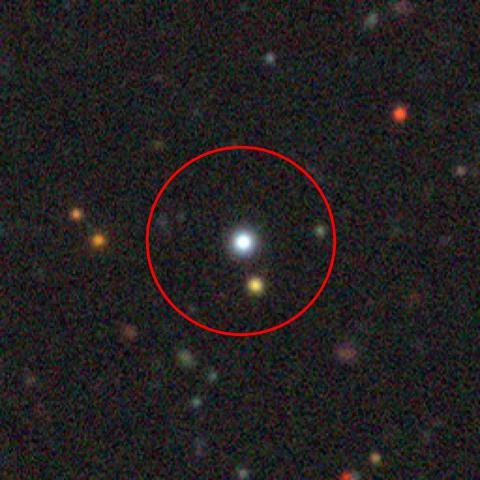
\includegraphics[width=\textwidth]{Images/ucds_exp/UCD_M87.png}
        \caption{}
    \end{subfigure}
    \begin{subfigure}[b]{0.3\textwidth}
        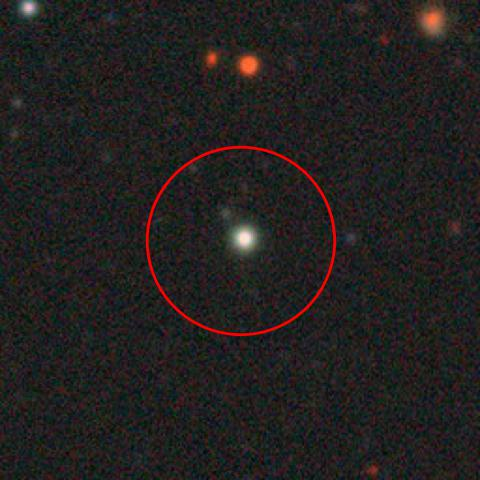
\includegraphics[width=\textwidth]{Images/ucds_exp/UCD_NGC1399.png}
        \caption{}
    \end{subfigure}
    \caption{Exemplos de galáxias anãs ultra-compactas encontradas em diferentes ambientes. a) UCD - Host M60, b) UCD - Host M87, c) UCD - Host NGC 1399. Créditos: a) Legacy Survey, b) Legacy Survey, c) Legacy Survey.}
    \label{UCDs_exp}
\end{figure}

\subsection{Propriedades UCDs}\label{subsec:propriedade}
As divisões sobre as UCDs, assim como parte das galáxias anãs, não seguem uma descrição estrita e definida uniformemente na literatura. Com os estudos sobre suas populações e diversidades, temos um intervalo médio de suas propriedades.

Quando comparadas com aglomerados globulares típicos, elas são mais largas, mais brilhantes e mais massivas. Os raios de meia-luz variam entre 10 e 100 parsecs ($10 \leq r_h \leq 100$ pc). Suas luminosidades estão na faixa de $-13 \leq M_g \leq -10$ magnitudes, em relação à magnitude absoluta na banda $g$.

As massas variam entre $10^6$ e $10^8$ massas solares ($M_{\odot}$) (\citealp{Mieske_2008_1}; \citealp{Misgeld_2011_2}) e o valor inferior é adotado para dividir o limite entre aglomerados estelares massivos e UCDs. Isso é feito por duas razões principais: Primeiro, sistemas estelares compactos começam a ter uma relação tamanho-luminosidade acima dessa massa (\citealp{Hasegan_2005}; \citealp{Cote_2006}; \citealp{Rejkuba_2007}; \citealp{Evstigneeva_2008}; \citealp{Norris_2011}), o que os distingue de aglomerados globulares, que têm tamanhos independentes da luminosidade \citep{Jornan_2005}. Isso provavelmente se deve à existência de uma densidade máxima de superfície estelar induzida por feedback estelar, possivelmente devido à evolução dinâmica e não à formação. Em segundo lugar, as proporções massa/luz dos sistemas estelares começam a aumentar além do previsto pelas populações estelares canônicas (\citealp{Hasegan_2005}; \citealp{Dabringhausen_2008}).

As UCDs apresentam predominantemente populações estelares mais antigas com um intervalo grande de metalicidades (\citealp{Evstigneeva_2009}; \citealp{Janz_2015}; \citealp{Zhang_2018}; \citealp{Forbes_2020}; \citealp{Fahrion_2020}). Elas têm dispersões de velocidade central entre os valores $20 < \sigma_0 < 50$ km s$^{-1}$ (\citealp{Hasegan_2005}; \citealp{Mieske_2008_1}), sendo $M-\sigma_0$ consistentes com a relação Faber-Jackson para a luminosidade de galáxias.

Além disso, elas têm em média uma razão de massa dinâmica para massa estelar de $M_{dyn}/M_* > 1$ ($M_{dyn}/M_* = 1.7 \pm 0.2$ para UCDs massivas com $M > 10^7 M_{\odot}$), enquanto para aglomerados globulares típicos, $M_{dyn}/M_* \approx 1$ \citep{Mieske_2013}.

Para a razão massa-luminosidade ($M/L$), que já foi estudada na literatura (\citealp{Hasegan_2005}; \citealp{Dabringhausen_2009}, \citeyear{Dabringhausen_2010}, \citeyear{Dabringhausen_2012}; \citealp{Baumgardt_2008}; \citealp{Mieske_2008_2}; \citealp{Taylor_2010}; \citealp{Frank_2011}; \citealp{Strader_2013}), e comparada com os modelos previstos para elas, observamos valores nas UCDs mais massivas que chegam a ser até 50\% maiores (\citealp{Hasegan_2005}; \citealp{Mieske_2008_2}). Quando comparadas com aglomerados globulares de metalicidades parecidas, elas chegam a ter $M/L$ 2 vezes maior, observadas na banda $v$. Foi sugerido que a presença de uma razão $M/L$ maior pode ser usada para distinguir UCDs de GCs. Porém, ainda assim é incerta a natureza dessa razão, ainda mais considerando que, por exemplo, \cite{Voggel_2018} sugere que a quantidade de UCDs com $M/L$ elevado pode estar sendo superestimada.

As explicações para $M/L$ maiores nas UCDs são muitas e podem ser atribuídas a uma combinação de motivos. As principais hipóteses dizem que isso pode ser devido à presença de matéria escura, uma variação na sua Função Inicial de Massa (IMF), a presença de buracos negros supermassivos ou perturbações causadas pela proximidade de uma galáxia massiva. Assim como suas formações, que possuem vários cenários possíveis, a razão elevada de $M/L$ também depende desses fatores.

\subsection{Cenários de Formação UCDs}\label{subsec:formacao}

Os cenários pelos quais as galáxias anãs ultra-compactas se formam ainda são debatidos, e diversas teorias são usadas para explicar sua origem. As mais aceitas seguem duas linhas principais: a primeira sugere que as UCDs são o resultado de galáxias anãs nucleadas que foram despojadas devido a interações gravitacionais, restando a UCD como o objeto final. A segunda linha sugere que as UCDs se formaram a partir de aglomerados estelares. O consenso mais aceito atualmente é que as UCDs fazem parte de uma família de objetos com mais de um cenário de origem.

Dentro desses cenários, podemos ainda ter algumas variações. Na ramificação dos GCs, temos a proposta de eles serem uma fusão de aglomerados estelares (\citealp{Kroupa_1998}; \citealp{Fellhauer_2002}; \citealp{Br_ns_2012}), ou surgindo diretamente como um aglomerado globular mais massivo próximo de galáxias em sistemas ricos desses objetos (\citealp{Mieske_2002}; \citealp{Mieske_2011}). Já na linha de galáxias despojadas, temos as teorias de serem sistemas, partes de um buraco negro supermassivo ejetados do centro de uma galáxia que retêm um denso aglomerado de estrelas (\citealp{Merritt_2009}; \citealp{Leigh_2013}). Ou uma das mais analisadas atualmente, sua formação a partir de núcleos despojados de galáxias anãs, que passaram por uma interação gravitacional, deixando apenas o núcleo restante como o objeto final (\citealp{Bassino_1994}; \citealp{Bekki_2001}; \citealp{Drinkwater_2003}; \citealp{Goerdt_2008}; \citealp{Pfeffer_2013}). Nas próximas subseções, falaremos um pouco dessas linhas de evolução desses objetos.

\subsubsection{Aglomerado globular}\label{subsubsec:}
Na linha de pensamento da origem das UCDs como aglomerados estelares, temos que eles podem ser aglomerados globulares muito massivos e luminosos, surgidos próximos a galáxias com sistemas ricos \citep{Mieske_2002}.

Elas podem surgir a partir da fusão de aglomerados globulares, em regiões mais densas em suas distribuições \citep{Fellhauer_2002}. Em simulações sobre as possíveis origens vindas de fusões de muitos aglomerados globulares \citep{Goerdt_2008}, vemos que é possível recriar as propriedades observadas nas UCDs, como suas massas, tamanhos e luminosidades. São necessários cerca de 50 GCs para produzir objetos que se assemelham às UCDs \citep{Goerdt_2008}. Essas fusões de GCs podem ser uma possível explicação do motivo de termos uma superdensidade local desses objetos próximos de alguns casos de UCDs \citep{Voggel_2016}.

Estudos comparativos das proporções de $M/L$ na banda $v$ com modelos de população estelar mostraram compatibilidade para UCDs nos aglomerados de Fornax \citep{Hilker_2006} e Virgem \citep{Evstigneeva_2007}. Em uma análise detalhada de uma das primeiras UCDs descobertas, a \textit{UCD3} em Fornax, \cite{Frank_2011} não encontrou evidências convincentes de matéria escura ou de um buraco negro central que pudesse aumentar a razão $M/L$. A dinâmica interna observada foi consistente com a de um aglomerado estelar massivo, reforçando a hipótese de que algumas UCDs podem se originar de aglomerados estelares.

\subsubsection{Galaxy stripping}\label{subsubsec:Galaxy stripping}

Na linha de raciocínio sobre a origem das UCDs, uma das mais estudadas é sua formação a partir de interações gravitacionais que despojam parte da galáxia inicial, formando esses objetos compactos.

Uma galáxia nucleada, após passar por fusões e interações, pode ter seu núcleo central sobrevivendo e permanecendo como um aglomerado luminoso \citep{Bassino_1994}. Exemplos vistos em \cite{Bekki_2001} mostram que, mesmo em várias passagens da galáxia original pela região central, as regiões externas foram removidas, mas o núcleo original foi pouco afetado, resultando em um objeto final com características semelhantes às UCDs.

Comparando com as simulações nesse cenário de formação, vemos que a distribuição de UCDs em aglomerados e galáxias é semelhante à encontrada nos modelos \citep{Thomas_2008}. A previsão, porém, indicou uma produção maior desses objetos em maiores raios, quando comparados com os dados observacionais. No entanto, esses modelos não levam em conta mudanças ao longo da trajetória desse aglomerado, como fusões de aglomerados menores ou outras interações.

Em \cite{Bekki_2003}, foi observado que a escala de tempo para que essa interação ocorra e forme esses objetos seria de bilhões de anos, com órbitas necessárias sendo bem excêntricas, exigindo que a galáxia hospedeira fosse mais luminosa do que magnitude $M_B = -16$. Tanto para órbitas elípticas, com mais passagens da galáxia original, quanto em órbitas mais caóticas, com poucas passagens, levam à formação de objetos semelhantes às UCDs, produzindo objetos nesse cenário que podem variar em luminosidade e tamanho do núcleo original. Assim, dependendo das interações, é possível formar vários tipos de objetos que observamos nas UCDs.

Após o processo de stripping, o núcleo muda pouco em sua estrutura, expandindo-se até 2-3 vezes seu tamanho, o que concorda com dados observacionais de que as UCDs são tipicamente 2 vezes maiores que o tamanho inicial do núcleo \citep{Evstigneeva_2008}.

\cite{Pfeffer_2016}, estudando as contribuições dos núcleos despojados na formação das UCDs, previram que o número de núcleos despojados escala com a massa viral do hospedeiro, sendo as UCDs de alta massa um grupo misto de formação de objetos e as de menores massas provavelmente vindas de origem de aglomerados globulares.

\cite{Pfeffer_2016} também previram as metalicidades de galáxias progenitoras de núcleos despojados e determinaram as metalicidades de seus núcleos. Eles compararam esses valores com as metalicidades observadas de aglomerados globulares e UCDs e concluíram que há uma boa concordância entre as metalicidades de UCDs e núcleos despojados para objetos com massa $M > 5 \times 10^6 M_{\odot}$.

Para comparar ainda melhor esses cenários, problemas como as resoluções de modelos semianalíticos e a falta da componente bariônica ainda se tornam um desafio. O estudo e a dificuldade da componente bariônica impactam tanto o tempo que as galáxias levam para passar pelo despojamento quanto o número de galáxias despojadas. Nesse caso, o uso de simulações hidrodinâmicas cosmológicas é necessário para obter melhores resultados, mas devido às resoluções para simulações das mesmas para galáxias anãs e de menores massas, ainda se torna um desafio. À medida que as UCDs se formam e se fundem em altos redshifts, é necessário um melhor entendimento de como os tempos e taxas de fusão evoluem para simulações precisas da formação de UCDs.

\subsubsection{Nuclear star clusters}\label{subsubsection:NSC}
Sobre a origem e os cenários de formação das UCDs, como parte da evolução desses objetos, discutidos no início desta seção sobre a possibilidade de terem se originado a partir de uma galáxia nucleada, vamos abordar um pouco sobre esse núcleo.

O núcleo está associado ao que é conhecido como \ac{NSC}. Eles são objetos compactos, massivos e mais luminosos quando comparados com os aglomerados globulares. Enquanto os aglomerados globulares estão na faixa de massa de $10^4$ até $10^6 M_{\odot}$ \citep{Masters_2010}, os NSCs estão na faixa de $10^6$ até $10^8 M_{\odot}$ (\citealp{Spengler_2017}; \citealp{Georgiev_2016}).

Suas detecções, devido às resoluções observacionais, em comparação ao próprio estudo da sua galáxia hospedeira, eram difíceis de separar nos primeiros estudos. Com a melhoria de novos instrumentos, com CCDs mais eficientes, conseguimos detectar e separar de maneira mais clara, encontrando-os tanto em galáxias early quanto late type (\citealp{Phillips_1996}; \citealp{Carollo_1997}; \citealp{Matthews_1999}; \citealp{boker_2002}).

Como parte da galáxia, os NSCs foram encontrados com relações semelhantes às de suas hospedeiras (\citealp{Balcells_2003}; \citealp{Graham_2003}). Algumas pesquisas estabeleceram relações entre a massa dos NSCs e propriedades da galáxia, como a luminosidade do bojo, dispersão de velocidade e massa estelar total (\citep{Ferrarese_2006};  \citep{Wehner_2006};  \citep{Rossa_2006}). Além disso, foi sugerido que os buracos negros e os NSCs seguem as mesmas relações de escala \citep{Ferrarese_2006}.

Sobre a quantidade de galáxias que hospedam um NSC, dada pela fração de nucleação, vemos que é alta. Segundo \cite{Boker_2010}, NSCs estão nos centros de mais de 70\% de todas as galáxias. No caso específico das galáxias anãs, analisaram galáxias no aglomerado de galáxias de Virgem como uma função da massa da galáxia \citep{Sanchez_2019}, para derivar a fração de nucleação delas. Concluíram que a fração de nucleação atinge o máximo em 90\% para galáxias com massas $M_{gal} \approx 10^9 M_{\odot}$, e cai constantemente para menos de 10\% para as massas de galáxias mais altas e mais baixas $M_{gal} < 10^6 M_{\odot}$ e $M_{gal} > 10^{11} M_{\odot}$, respectivamente.

Para as galáxias anãs menos massivas ($M_{gal} < 10^6 M_{\odot}$), a fração de nucleação é próxima de zero \citep{Ordenes_2018}. Além disso, são escassos os aglomerados globulares (GCs) nessas galáxias \citep{Forbes_2018}, o que pode indicar que esses objetos não são capazes de formar aglomerados estelares massivos. Para as galáxias anãs mais massivas, foi sugerido que as interações entre os aglomerados estelares nucleares (NSCs) e os buracos negros supermassivos (SMBHs) centrais podem interromper os NSCs existentes ou inibir diretamente a formação de novos NSCs (\citealp{Cote_2006}; \citealp{Neumayer_2012}; \citealp{Antonini_2015}; \citealp{Arca_2016}).

Foram encontrados vários casos onde coexistiam o buraco negro supermassivo na galáxia com a presença de um NSC \citep{Graham_2009}. Em relação à fração de massa entre o buraco negro e a massa do NSC, a fração de massa aumenta com a massa da galáxia e, portanto, os buracos negros começam a dominar a parcela de massa central para galáxias mais massivas do que $3 \times 10^{10} M_{\odot}$. Esses podem ser sistemas onde o buraco negro supermassivo começa a afetar o crescimento do NSC devido a fusões binárias de buracos negros e interações dinâmicas com as estrelas do NSC \citep{Antonini_2015}. Já para galáxias menores, a massa do NSC domina.

Como estudo da evolução das galáxias com a presença de NSCs, estudos como o de \cite{Wang_2023} investigaram a continuidade na evolução desses objetos. Eles mapearam as galáxias no aglomerado de Virgem, encontrando objetos com morfologias transitórias.

\noindent Eles explicam a evolução contínua de formação dos seguintes objetos:

Galáxias anãs elípticas nucleadas (dE,N) - São galáxias anãs elípticas que possuem um aglomerado estelar nuclear. Algumas delas são fortemente nucleadas, apresentando uma fração de luminosidade nuclear maior do que a média.

Galáxias anãs elípticas nucleadas com envelopes estendidos (eUCDs - extended Ultra-Compact Dwarfs) - Representam um estágio intermediário entre as dE,Ns e as UCDs, apresentando envelopes estelares detectáveis.

Galáxias anãs ultra-compactas – Sistemas compactos com raios de meia-luz entre 10 e 100 parsecs, que podem ser núcleos remanescentes de galáxias anãs que passaram por um forte processo de stripping tidal.

Na Figura \ref{continuo_evolution_dwarf}, mostramos os tipos de galáxias explicadas no trabalho de \cite{Wang_2023}, que exemplificam o contínuo de evolução esperado entre os objetos que podem ter passado pelo processo de tidal stripping, levando galáxias anãs nucleadas a se transformarem até o ponto de UCDs. A figura mostra alguns representantes das classes do contínuo de evolução aplicadas. Da esquerda para a direita, temos uma galáxia anã com a presença de um NSC, seguida por uma galáxia passando pelo processo de tidal stripping, ainda nucleada, mas com o envoltório nuclear mostrando sinais de interação com galáxias massivas próximas. Depois, temos uma galáxia categorizada como ultra-difusa (\ac{UDG}), com um envoltório nuclear ainda bem detectável, mas extenso e fraco. Logo depois, temos uma galáxia categorizada como fortemente nucleada, quando categorizadas de acordo com a fração de luminosidade comparada entre o núcleo e o envoltório. Por último, temos duas galáxias que seriam detectáveis como UCDs, uma com um centro envoltório ainda presente e outra mais pontual, como apenas o remanescente final do NSC.

\begin{figure}[!ht]
    \centering
    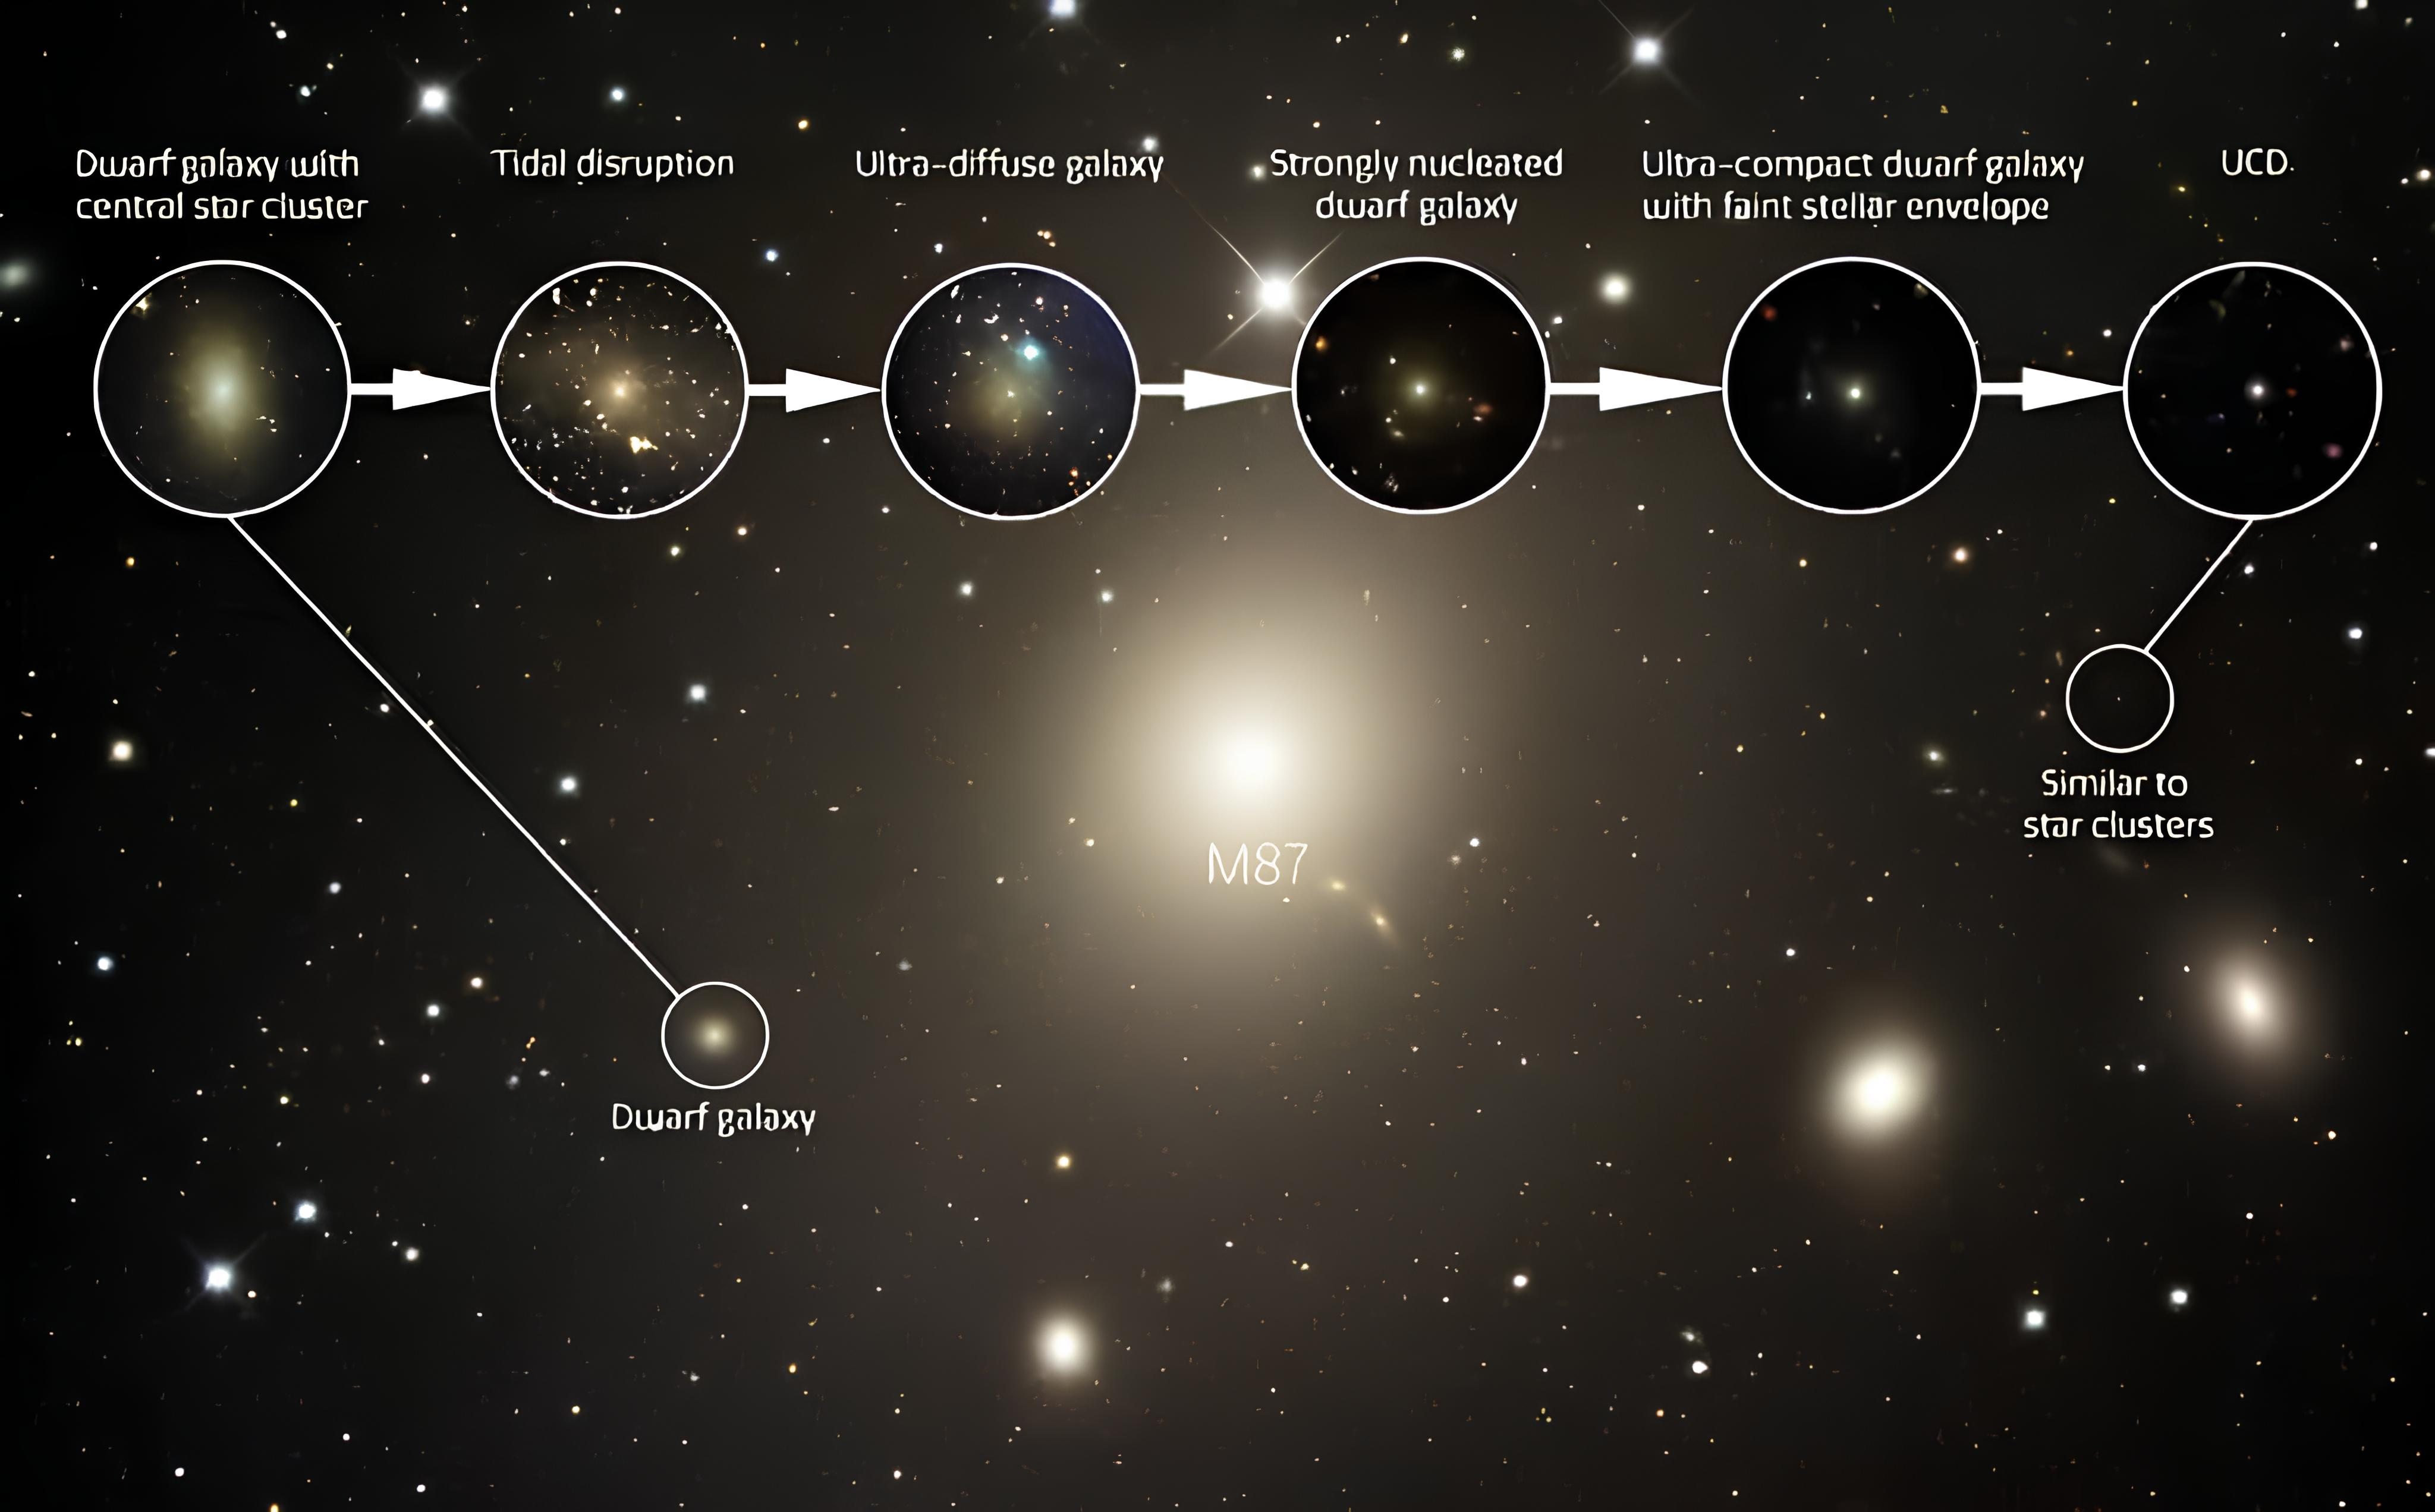
\includegraphics[width=1.\columnwidth,angle=0]{continuo_evolution_dwarf.png} 
    \caption[]{Um contínuo de galáxias capturadas em diferentes estágios do processo de transformação de uma galáxia anã em uma anã ultra-compacta (UCD). Esses objetos estão localizados perto da supergigante M87, o membro dominante do vizinho Aglomerado de Virgem. Crédito: NOIRLab/NSF/AURA/NASA/R. Gendler/K. Wang/M. Zamani}
    \label{continuo_evolution_dwarf}
\end{figure}

\subsection{Espectroscopia em UCDs}\label{subsec:espectroscopia}
A espectroscopia para as galáxias no universo localizados é fundamental para entender a sua história de formação estelar, juntamente com a evolução química e dinâmica interna. A espectroscopia de galáxias anãs permite determinar as velocidades radiais individuais de estrelas, que, por sua vez, são utilizadas para modelar a distribuição de massa e inferir os perfis de matéria escura em sistemas de baixa massa. Estudos pioneiros demonstraram que as UCDs apresentam perfis de velocidade internos distintos tanto de aglomerados globulares quanto de galáxias nucleadas, sugerindo mais de um cenário de formação \citep{Drinkwater_2003, Bekki_2003}. 

As principais aplicações que a espectroscopia pode trazer para o estudo das galáxias anãs ultra-compactas envolvem o estudo da cinemática e dinâmica. A dispersão de velocidade interna, obtida de linhas de absorção, fornece estimativas de massas dinâmicas e frações de matéria escura \citep{Chilingarian_2011}. Observações com o Gemini/GMOS de UCDs no grupo fóssil NGC 1132 confirmaram a presença de seis UCDs com velocidades radiais médias e dispersão de velocidades comparáveis aos de grupos de galáxias pobres \citep{Madrid_2013}.

As UCDs exibem espectros dominados por linhas de absorção. Linhas proeminentes como o triplete de Ca II, Mg b e Fe são frequentemente observadas, indicando a presença de estrelas velhas e uma metalicidade relativamente alta. Estudos espectroscópicos, como o realizado por \cite{Mieske_2006}, revelaram uma quebra na distribuição de metalicidade em torno de $M_V \approx -11$ mag, sugerindo diferentes origens para UCDs mais brilhantes em comparação com aglomerados globulares. Assim, os estudos dos índices espectrais e dos ajustes de síntese de populações permitiram reconstruir as histórias de formação e distinguir as UCDs formadas por galáxias nucleadas que foram despojadas de aglomerados globulares massivos \citep{Mieske_2006}.

Dessas mesmas análises de \cite{Mieske_2006}, comparações entre os espectros de UCDs e aglomerados globulares mostram que, embora compartilhem algumas características, UCDs tendem a apresentar linhas de absorção mais intensas e larguras de linha maiores, refletindo suas maiores massas e possíveis histórias de formação distintas.

Assim, os espectros das UCDs são predominantemente compostos por linhas de absorção, refletindo suas populações estelares antigas e metalicamente enriquecidas. A presença de linhas de emissão é rara e, quando observada, pode indicar atividade de formação estelar recente ou núcleos ativos fracos.

\section{Galáxias compactas com emissão}\label{sec:galaxias_compactas_emissao}
As galáxias anãs ultra-compactas e as Blue Compact Dwarf galaxies são objetos distintos, com propriedades e cenários de formação diferentes. No entanto, durante este trabalho de busca por UCDs, nosso método identificou algumas galáxias que podem ser classificadas como BCDs, as quais são mencionadas no Capítulo 5. Nesta seção, discutiremos brevemente suas características e relevância.

As BCDs são particularmente interessantes para o estudo de ambientes de formação estelar intensa em condições de baixa metalicidade. Seus espectros são dominados por linhas de emissão, como H$\alpha$, H$\beta$, [O III] $\lambda 5007$, [O II] $\lambda 3727$, [N II] $\lambda 6584$ e [S II] $\lambda 6717$, que refletem a presença de regiões H II ionizadas por estrelas jovens e massivas. Além disso, estudos no infravermelho próximo revelaram linhas de emissão de hidrogênio molecular (H$2$), hélio e ferro, sugerindo processos adicionais, como excitação fluorescente e choques \citep{Izotov_2011}. Em alguns casos, a presença de linhas de emissão amplas pode ser atribuída a ventos estelares, supernovas ou, raramente, à atividade de núcleos galácticos ativos \citep{Izotov_2007}.

A formação das BCDs está intimamente ligada a processos dinâmicos e evolutivos. Simulações numéricas indicam que a fusão entre galáxias anãs ricas em gás pode desencadear starbursts centrais, formando núcleos compactos dominados por populações estelares jovens, enquanto as componentes estelares antigas dos progenitores tornam-se envoltórios de baixa luminosidade superficial \citep{Bekki_2008}. Em ambientes de aglomerados, interações com o meio intraaglomerado (ICM) ou com outras galáxias podem comprimir o gás interestelar, desencadeando starbursts. Estudos de \citep{Watts_2016} sugerem que, após a remoção do gás e a cessação da formação estelar, BCDs em aglomerados, como os da periferia do aglomerado de Virgem, podem evoluir para galáxias anãs elípticas.

Modelos de evolução química propõem que as BCDs podem experimentar regimes de formação estelar contínua ou intermitente (bursting ou gasping). No cenário gasping, períodos de formação estelar ativa são separados por intervalos de inatividade mais curtos que os períodos ativos. Esses modelos, que consideram uma eficiência moderada de formação estelar e ventos galácticos enriquecidos em metais, conseguem reproduzir as abundâncias químicas observadas em BCDs \citep{Yin_2011}.

Portanto, a formação e evolução das BCDs são influenciadas por uma combinação de processos, como fusões de galáxias anãs, interações em ambientes densos e diferentes regimes de formação estelar. Enquanto as UCDs apresentam espectros dominados por linhas de absorção, refletindo populações estelares antigas e inativas em termos de formação estelar, as BCDs exibem espectros ricos em linhas de emissão, evidenciando formação estelar ativa e recente. Essa distinção espectral destaca os diferentes estágios evolutivos e mecanismos de formação entre esses dois tipos de galáxias.




% \subsection{Buracos negros em UCDs}\label{subsec:buracos negros}
% A presença de buracos negros em UCDs é fundamental para avaliar a relevância dos diferentes processos de formação dessas galáxias e para compreender a densidade de buracos negros supermassivos (SMBH) no universo local \citep{Seth_2014}.

% A presença de buracos negros e seu estudo são importantes para entender os mecanismos de evolução das galáxias. Em simulações, vemos que as galáxias de menor massa surgem mais cedo do que o esperado \citep{Weinmann_2012}. O papel dos buracos negros nessas galáxias pode ajudar a explicar parte dessa questão, pois eles têm propriedades ligadas à sua galáxia hospedeira, como a dispersão de velocidade.

% Eles têm um papel importante na regulação da formação estelar de uma galáxia, devido aos processos de feedback, que podem impulsionar suas transformações. O papel desses feedbacks é ajustado em simulações para observar as medidas vistas no universo, pois as resoluções das simulações para essas galáxias não são profundas o suficiente para estudá-los diretamente \citep{Springel_2005}.

% Sobre as relações de escala, comparadas com as galáxias mais massivas, observa-se que as de menor massa têm uma relação mais íngreme. Esse resultado pode ser uma consequência de um viés das medições indiretas de buracos negros nas galáxias de baixa massa, quando comparadas com os melhores dados diretos de outras mais massivas \citep{Shankar_2016}. Esse resultado também pode ser uma consequência direta dos próprios mecanismos de formação dessas galáxias, que mudam suas relações de escala. No início de suas vidas, seu crescimento é principalmente induzido pela acreção de gás, mudando depois para fusões ao longo do tempo \citep{Graham_2015}.


% \section{Questões em aberto}\label{sec:Questoes_abertas}

% Embora os estudos sobre as UCDs tenham avançado significativamente nos últimos anos, sua origem e evolução ainda são temas de intenso debate. Diversos cenários foram propostos para explicar sua formação, sendo o stripping tidal de galáxias anãs um dos mais aceitos. No entanto, os modelos clássicos de stripping frequentemente negligenciam o papel das fusões hierárquicas em ambientes de aglomerados, onde pequenas subestruturas podem contribuir para a população final de UCDs. 




% Além disso, abordagens semi-analíticas, apesar de fornecerem insights valiosos, carecem de um tratamento adequado da componente bariônica, que influencia diretamente os processos dinâmicos e os tempos de stripping.

% Diante dessas limitações, as simulações hidrodinâmicas cosmológicas emergem como uma ferramenta essencial para investigar a formação e a distribuição das UCDs no contexto da evolução das galáxias em aglomerados. Essas simulações permitem obter previsões mais robustas sobre a frequência de núcleos despojados e a relação entre UCDs e seus progenitores. Neste capítulo, discutimos algumas das principais questões em aberto sobre a natureza das UCDs e os desafios que permanecem para a compreensão de sua formação e evolução.



